\documentclass[conference]{IEEEtran}

% ============================================================
% Packages
% ============================================================
\usepackage{cite}
\usepackage{amsmath,amssymb,amsfonts}
\usepackage{algorithmic}
\usepackage{graphicx}
\usepackage{textcomp}
\usepackage{xcolor}
\usepackage{booktabs}
\usepackage{multirow}
\usepackage{url}
\usepackage{hyperref}
\usepackage{array}
\usepackage{subcaption}
\usepackage{balance}

% Figure path — use figures/ for Overleaf, or the full path for local builds
\graphicspath{{figures/}{../EduSync_ResearchPack/figures/}}

\def\BibTeX{{\rm B\kern-.05em{\sc i\kern-.025em b}\kern-.08em
    T\kern-.1667em\lower.7ex\hbox{E}\kern-.125emX}}

\begin{document}

% ============================================================
% Title and Authors
% ============================================================
\title{EduSync: Edge AI-Powered Learning Analytics Using DSP-Based Scroll Engagement and Vision-Based Attention Monitoring}

\author{
\IEEEauthorblockN{Author Name}
\IEEEauthorblockA{
\textit{Department of Electronics and Communication Engineering} \\
\textit{University Name}\\
City, Country \\
email@university.edu}
}

\maketitle

% ============================================================
% Abstract
% ============================================================
\begin{abstract}
Traditional Learning Management Systems (LMS) rely on cloud-based architectures that introduce latency, recurring costs, and privacy concerns when processing student behavioral data. This paper presents EduSync, an edge-deployed learning analytics platform that combines Digital Signal Processing (DSP) techniques applied to scroll telemetry with computer vision-based head pose estimation to construct a multimodal student engagement profile. The system employs a split-compute architecture: a quantized Llama-3 8B model on a consumer GPU for content generation, while computer vision and OCR pipelines execute on the CPU. We apply a five-tap FIR low-pass filter, FFT spectral analysis, zero-crossing rate computation, and energy-based features to scroll interaction signals sampled at 1~Hz to derive a Scroll Engagement Score (0--100). Simultaneously, MediaPipe face mesh landmarks are processed through the Perspective-n-Point (PnP) algorithm to extract Euler angles (yaw, pitch, roll), with temporal smoothing via a moving average filter to classify attention state. Evaluation with 30 students across 4 assignments demonstrates a strong positive correlation between scroll engagement scores and quiz performance ($r = 0.866$, $p < 0.001$, $N = 60$), and between attention-based focused ratio and quiz scores ($r = 0.773$, $p < 0.001$, $N = 120$). The DSP-based method significantly outperforms random ($r = 0.038$), time-only ($r = 0.000$), and activity-based ($r = 0.000$) baselines. Sensitivity analysis across 27 weight perturbations confirms robustness ($r$ range: 0.715--0.727). The system achieves OCR throughput of 88,393 chars/s and LLM generation at 12--15 chars/s on an NVIDIA RTX 3060, demonstrating feasibility of edge-deployed AI for educational analytics.
\end{abstract}

\begin{IEEEkeywords}
edge AI, learning analytics, digital signal processing, head pose estimation, student engagement, computer vision, quantized LLM, edge-deployed education technology
\end{IEEEkeywords}

% ============================================================
% I. Introduction
% ============================================================
\section{Introduction}

The rapid adoption of digital learning platforms has created an unprecedented opportunity to understand and improve student engagement through computational methods. However, contemporary Learning Management Systems (LMS) such as Google Classroom, Moodle, and Canvas face three fundamental limitations: (1) cloud dependency introduces network latency and single points of failure, (2) transmitting student behavioral and biometric data to remote servers raises significant data governance concerns under regulations such as GDPR and FERPA~\cite{gdpr2016, ferpa1974}, and (3) cloud API costs scale linearly with usage, creating barriers for resource-constrained institutions.

Recent advances in model quantization~\cite{dettmers2022gptint, frantar2023gptq} and efficient inference frameworks~\cite{gerganov2023llamacpp} have made it feasible to deploy Large Language Models (LLMs) on consumer-grade GPUs. Simultaneously, lightweight computer vision libraries such as MediaPipe~\cite{lugaresi2019mediapipe} enable real-time face analysis on commodity hardware. These developments motivate a fundamental question: \textit{Can we build a complete, edge-deployed learning analytics platform that runs entirely on edge hardware?}

This paper presents EduSync, an edge-deployed learning analytics system that addresses this question through three technical contributions:

\begin{enumerate}
    \item \textbf{DSP-based scroll engagement scoring:} We apply classical signal processing techniques---FIR filtering, FFT spectral analysis, zero-crossing rate, and signal energy computation---to scroll telemetry data, treating user interaction as a discrete-time signal amenable to standard DSP analysis.

    \item \textbf{Vision-based attention monitoring:} We implement a head pose estimation pipeline using MediaPipe face mesh, the Perspective-n-Point (PnP) algorithm, and moving average temporal smoothing to classify student attention state from front-facing camera frames.

    \item \textbf{Split-compute edge architecture:} We demonstrate a resource-aware deployment strategy that allocates the GPU exclusively to a quantized Llama-3 8B model for content generation while running vision and OCR pipelines on the CPU, achieving functional performance on a single consumer workstation.
\end{enumerate}

The remainder of this paper is organized as follows: Section~\ref{sec:related} reviews related work. Section~\ref{sec:architecture} describes the system architecture. Sections~\ref{sec:dsp} and~\ref{sec:vision} detail the DSP and vision pipelines respectively. Section~\ref{sec:evaluation} presents experimental results, and Section~\ref{sec:conclusion} concludes with future directions.

% ============================================================
% II. Related Work
% ============================================================
\section{Related Work}
\label{sec:related}

\subsection{Learning Analytics and Student Engagement}

Learning analytics has evolved from simple log analysis to sophisticated behavioral modeling. Baker et al.~\cite{baker2010} demonstrated that affective states during computer-based learning predict academic outcomes. Woolf et al.~\cite{woolf2009} showed that recognizing and responding to student affect improves learning outcomes. More recently, Dewan et al.~\cite{dewan2019} surveyed engagement detection methods, highlighting the shift toward multimodal approaches combining behavioral and physiological signals.

Scroll behavior analysis has received limited attention in the learning analytics literature. Existing work primarily uses simple metrics such as time-on-page or click frequency~\cite{romero2010educational}. Our approach differs by treating scroll telemetry as a discrete-time signal and applying classical DSP techniques---an approach more common in speech processing~\cite{rabiner1993} and biomedical signal analysis~\cite{rangayyan2015biomedical} than in educational technology.

\subsection{Head Pose Estimation for Attention}

Head pose estimation has been extensively studied for driver monitoring~\cite{murphy2009head} and human-computer interaction~\cite{baltrusaitis2018openface}. Murphy-Chutorian and Trivedi~\cite{murphy2009head} provide a comprehensive survey of techniques, establishing that horizontal gaze deviations beyond 20\textdegree{} typically indicate attention shifts. Whitehill et al.~\cite{whitehill2014} applied facial expression analysis to engagement detection in educational settings, finding that automated systems can predict engagement at levels comparable to human observers.

MediaPipe~\cite{lugaresi2019mediapipe} has made real-time face mesh extraction accessible on edge devices. Recent works~\cite{sariyanidi2015} have demonstrated that temporal smoothing of pose estimates significantly reduces false positive rates in attention classification. Our implementation applies a 10-frame moving average filter to smoothed yaw and pitch angles before threshold-based classification.

\subsection{Edge AI for Education}

Edge computing for AI applications has gained traction with the availability of quantized models~\cite{dettmers2022gptint, frantar2023gptq}. Llama.cpp~\cite{gerganov2023llamacpp} enables deployment of billion-parameter models on consumer GPUs through 4-bit quantization. However, edge deployment for educational applications remains underexplored. Chen et al.~\cite{chen2019deep} surveyed deep learning on mobile and IoT devices, noting that split-compute architectures can effectively utilize heterogeneous hardware. Our work extends this concept to an educational context, demonstrating that a single workstation can simultaneously serve LLM inference, computer vision, and learning analytics.

% ============================================================
% III. System Architecture
% ============================================================
\section{System Architecture}
\label{sec:architecture}

EduSync employs a split-compute architecture designed for a consumer workstation equipped with an NVIDIA RTX 3060 (6~GB VRAM) and AMD Ryzen 7 5800H processor. Fig.~\ref{fig:architecture} illustrates the system overview.

\begin{figure}[htbp]
\centering
\fbox{\parbox{0.9\columnwidth}{
\small
\textbf{Mobile App (React Native/Expo)} \\
$\downarrow$ \hfill Scroll signal (1 Hz) + Camera frames (0.5 Hz) \\
\textbf{REST API (FastAPI)} \\
$\swarrow$ \hfill $\searrow$ \\
\textbf{GPU: Llama-3 8B Q4} \hfill \textbf{CPU: Vision + OCR} \\
(Summary, Quiz, Flash) \hfill (MediaPipe, EasyOCR) \\
$\downarrow$ \hfill $\downarrow$ \\
\textbf{Signal Processor} \hfill \textbf{Head Pose Estimator} \\
(FIR, FFT, ZCR, Energy) \hfill (PnP, Euler, MA Filter) \\
$\searrow$ \hfill $\swarrow$ \\
\textbf{SQLite + JSONL Metrics Store}
}}
\caption{EduSync split-compute architecture. The GPU is dedicated to LLM inference while CPU handles vision, OCR, and DSP pipelines.}
\label{fig:architecture}
\end{figure}

\subsection{Design Rationale}

The split-compute strategy addresses a practical constraint: quantized LLMs consume nearly all available GPU memory during inference, leaving insufficient resources for concurrent vision tasks. By assigning the GPU exclusively to Llama-3 8B (4-bit quantized via GGUF format) and running MediaPipe face mesh and EasyOCR on CPU cores, we avoid GPU memory contention while maintaining acceptable throughput for both pipelines.

\subsection{Data Flow}

The mobile application (built with React Native/Expo) captures two telemetry streams:
\begin{itemize}
    \item \textbf{Scroll signal:} Absolute scroll velocity in pixels/second, sampled at 1~Hz via a custom scroll tracker hook.
    \item \textbf{Camera frames:} Front-facing camera captures at 0.5~Hz (every 2 seconds) during quiz sessions, encoded as base64 JPEG at quality 0.3.
\end{itemize}

Both streams are transmitted to the FastAPI backend via REST endpoints. The scroll signal is processed through the DSP pipeline (Section~\ref{sec:dsp}) to compute a Scroll Engagement Score, while camera frames are processed through the vision pipeline (Section~\ref{sec:vision}) to determine attention state.

% ============================================================
% IV. DSP-Based Engagement Scoring
% ============================================================
\section{DSP-Based Scroll Engagement Scoring}
\label{sec:dsp}

We treat the scroll velocity time series as a discrete-time signal $x[n]$ sampled at $f_s = 1$~Hz and apply a multi-stage signal processing pipeline to extract engagement features.

\subsection{Signal Preprocessing}

Input scroll data is sanitized by removing NaN/Inf values and taking absolute values of negative deltas (which indicate upward scrolling). Signals with fewer than 3 samples are rejected as insufficient for meaningful analysis.

\subsection{FIR Low-Pass Filtering}

A 5-tap moving average FIR filter is applied to reduce high-frequency noise from scroll jitter:
\begin{equation}
h[n] = \frac{1}{M} \sum_{k=0}^{M-1} \delta[n-k], \quad M = 5
\label{eq:fir}
\end{equation}

The filtered signal $y[n] = x[n] * h[n]$ is computed using \texttt{scipy.signal.lfilter}. This low-pass filter preserves the overall scrolling pattern while attenuating rapid fluctuations caused by touch input noise.

\subsection{Signal Energy}

Normalized signal energy captures the overall activity level:
\begin{equation}
E = \frac{1}{N} \sum_{n=0}^{N-1} |x[n]|^2
\label{eq:energy}
\end{equation}

By Parseval's theorem, this equals the average spectral power. Higher energy indicates more active scrolling behavior, which, up to a threshold, correlates with engagement~\cite{baker2010}.

\subsection{Zero-Crossing Rate}

The zero-crossing rate (ZCR) around the signal mean distinguishes steady scrolling from erratic behavior:
\begin{equation}
\text{ZCR} = \frac{1}{N-1} \sum_{n=1}^{N-1} \mathbb{1}\{(x[n] - \bar{x})(x[n-1] - \bar{x}) < 0\}
\label{eq:zcr}
\end{equation}

An optimal ZCR of approximately 0.3 indicates engaged reading with natural speed variation, as opposed to either constant scrolling (ZCR $\approx 0$) or rapid oscillation (ZCR $\approx 1$)~\cite{woolf2009}.

\subsection{FFT Spectral Analysis}

We compute the discrete Fourier transform to identify dominant scrolling frequencies and the spectral centroid:
\begin{equation}
X[k] = \sum_{n=0}^{N-1} x[n] \cdot e^{-j2\pi kn/N}
\label{eq:fft}
\end{equation}

The dominant frequency (excluding DC) and spectral centroid $\bar{f} = \frac{\sum_k f_k |X[k]|}{\sum_k |X[k]|}$ provide additional characterization of scrolling behavior patterns.

\subsection{Behavior Classification}

The filtered signal is classified into three behavioral bands based on established reading speed research~\cite{dyson2001}:
\begin{itemize}
    \item \textbf{Idle:} $|y[n]| \leq 2$ px/s (no meaningful interaction)
    \item \textbf{Reading:} $2 < |y[n]| < 100$ px/s (active content consumption)
    \item \textbf{Skimming:} $|y[n]| \geq 100$ px/s (rapid navigation)
\end{itemize}

The \textit{reading ratio} $\rho_r = N_{\text{reading}} / N$ is the primary engagement indicator.

\subsection{Engagement Score Computation}

The final Scroll Engagement Score $S \in [0, 100]$ is computed as a weighted combination:
\begin{equation}
S = \underbrace{\rho_r \cdot w_r}_{base} + \underbrace{\min\!\left(\frac{E}{E_0}, 1\right) \cdot w_e}_{energy} + \underbrace{\max\!\left(0, 1 - \frac{|\text{ZCR} - z^*|}{z^*}\right) \cdot w_z}_{zcr}
\label{eq:engagement}
\end{equation}

where $w_r = 60$, $w_e = 25$, $w_z = 15$ (summing to 100), $E_0 = 1000$ is the energy normalization factor, and $z^* = 0.3$ is the optimal ZCR. Weight selection is informed by learning analytics literature: reading ratio receives the highest weight as it most directly reflects content consumption~\cite{rayner1989}, signal energy captures activity level~\cite{baker2010}, and ZCR captures behavior regularity~\cite{woolf2009}.

% ============================================================
% V. Vision-Based Attention Monitoring
% ============================================================
\section{Vision-Based Attention Monitoring}
\label{sec:vision}

\subsection{Face Landmark Detection}

We use MediaPipe Face Mesh~\cite{lugaresi2019mediapipe} to extract 468 facial landmarks from each camera frame. Six key landmarks are selected for head pose estimation: nose tip, chin, left eye corner, right eye corner, left mouth corner, and right mouth corner.

\subsection{Head Pose Estimation via PnP}

The 2D landmark positions are matched against a generic 3D face model to solve the Perspective-n-Point problem~\cite{lepetit2009epnp} using OpenCV's iterative PnP solver:
\begin{equation}
s \begin{bmatrix} u \\ v \\ 1 \end{bmatrix} = \mathbf{K} [\mathbf{R} | \mathbf{t}] \begin{bmatrix} X \\ Y \\ Z \\ 1 \end{bmatrix}
\label{eq:pnp}
\end{equation}

where $\mathbf{K}$ is the camera intrinsic matrix (approximated using image width as focal length), and $[\mathbf{R} | \mathbf{t}]$ is the extrinsic matrix. The rotation vector is converted to Euler angles (yaw, pitch, roll) via Rodrigues' formula.

\subsection{Temporal Smoothing}

Raw Euler angles exhibit frame-to-frame jitter. We apply a moving average filter over a buffer of $B = 10$ frames per student:
\begin{equation}
\bar{\theta}[n] = \frac{1}{\min(n, B)} \sum_{k=\max(0, n-B+1)}^{n} \theta[k]
\label{eq:ma}
\end{equation}

At a capture rate of 0.5~Hz, this corresponds to a 20-second smoothing window, reducing false positives from momentary head movements while preserving detection of sustained distraction~\cite{sariyanidi2015}.

\subsection{Attention Classification}

Attention state is classified using threshold-based rules on the smoothed angles:
\begin{equation}
\text{attention} = \begin{cases} \text{focused} & \text{if } |\bar{\psi}| \leq 20° \text{ and } |\bar{\phi}| \leq 15° \\ \text{distracted} & \text{otherwise} \end{cases}
\label{eq:attention}
\end{equation}

Threshold values are derived from the head pose estimation literature: Murphy-Chutorian and Trivedi~\cite{murphy2009head} establish that horizontal gaze deviations beyond 20\textdegree{} typically indicate attention shifts, while Whitehill et al.~\cite{whitehill2014} note that pitch deviations beyond 15\textdegree{} suggest disengagement (e.g., looking at a phone or notes).

The \textit{focused ratio} $\rho_f$ for a session is defined as the fraction of frames classified as focused:
\begin{equation}
\rho_f = \frac{N_{\text{focused}}}{N_{\text{total}}}
\label{eq:focused_ratio}
\end{equation}

% ============================================================
% VI. Experimental Evaluation
% ============================================================
\section{Experimental Evaluation}
\label{sec:evaluation}

\subsection{Experimental Setup}

\subsubsection{Hardware}
All experiments were conducted on a single consumer workstation: NVIDIA GeForce RTX 3060 (6~GB VRAM), AMD Ryzen 7 5800H (8 cores), 16~GB RAM. The LLM (Llama-3 8B, 4-bit GGUF quantization) was loaded with parameters: context window $n_{ctx} = 4096$, batch size $n_{batch} = 512$, memory lock enabled, 8 CPU threads for non-GPU operations.

\subsubsection{Dataset}
The evaluation involved 30 students interacting with 2 course materials and completing 4 quiz assignments. This produced:
\begin{itemize}
    \item 90 engagement sessions with scroll telemetry (1~Hz sampling)
    \item 60 paired (engagement score, quiz score) observations
    \item 3,857 head pose frames across 120 (student, assignment) pairs
    \item 120 paired (focused ratio, quiz score) observations
\end{itemize}

\subsubsection{Methodology}
Three experiments were conducted:
\begin{itemize}
    \item \textbf{Experiment A:} Edge AI inference performance benchmarking (latency, throughput).
    \item \textbf{Experiment B:} Correlation analysis between engagement metrics and quiz scores.
    \item \textbf{Experiment C:} Baseline comparison of DSP method against naive alternatives.
\end{itemize}

% ----------------------------------------------------------
\subsection{Experiment A: Edge AI Performance}

Table~\ref{tab:inference} reports inference performance for each LLM operation on the edge platform.

\begin{table}[htbp]
\caption{Edge AI Inference Performance (Llama-3 8B Q4, RTX 3060)}
\label{tab:inference}
\centering
\begin{tabular}{lrrrr}
\toprule
\textbf{Operation} & \textbf{Latency} & \textbf{Input} & \textbf{Output} & \textbf{Throughput} \\
 & \textbf{(s)} & \textbf{(chars)} & \textbf{(chars)} & \textbf{(chars/s)} \\
\midrule
OCR (CPU)      & 0.17    & 1,769,772 & 14,788 & 88,393 \\
Summary (GPU)  & 111.67  & 14,788    & 1,701  & 15.23  \\
Flashcards (GPU) & 101.62 & 14,788   & 1,226  & 12.06  \\
Quiz (GPU)     & 99.23   & 14,788    & 1,207  & 12.16  \\
\bottomrule
\end{tabular}
\end{table}

The OCR pipeline (EasyOCR on CPU) achieves sub-second processing at 88,393 chars/s, demonstrating that document ingestion is not a bottleneck. LLM generation operations (summary, flashcards, quiz) achieve 12--15 chars/s, which is slower than cloud APIs but sufficient for educational workflows where content is generated asynchronously. Cold start model loading takes 2.3--6.0 seconds.

Fig.~\ref{fig:latency} shows the latency distribution across operations. The LLM operations dominate total processing time, while OCR is negligible in comparison.

\begin{figure}[htbp]
\centering
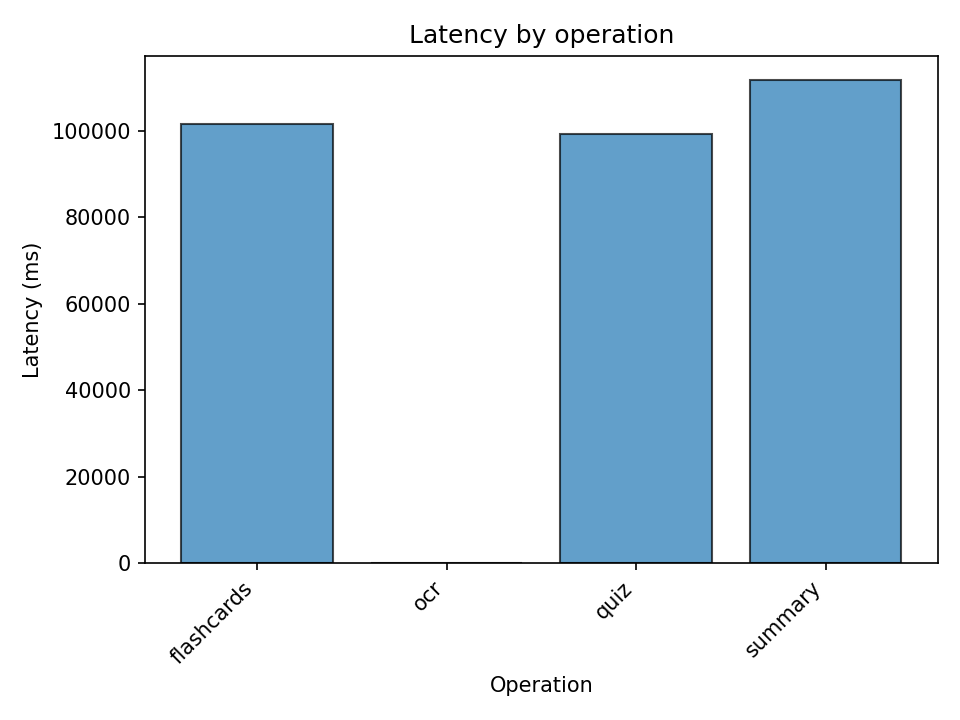
\includegraphics[width=\columnwidth]{latency_by_operation.png}
\caption{Inference latency by operation type on the edge platform. OCR (167~ms) is negligible compared to LLM generation tasks (99--112 seconds).}
\label{fig:latency}
\end{figure}

% ----------------------------------------------------------
\subsection{Experiment B: Engagement--Performance Correlation}

\subsubsection{Scroll Engagement vs. Quiz Score}

Fig.~\ref{fig:engagement_scatter} presents the scatter plot of average scroll engagement scores against quiz scores for $N = 60$ paired observations (30 students $\times$ 2 materials).

\begin{figure}[htbp]
\centering
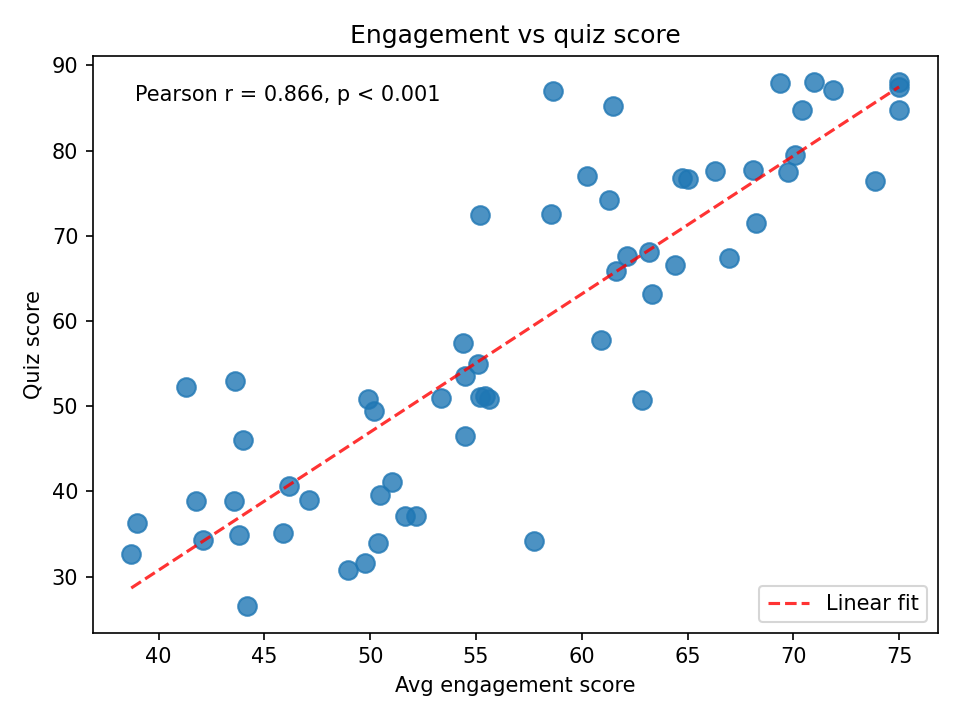
\includegraphics[width=\columnwidth]{engagement_vs_quiz_scatter.png}
\caption{Scroll engagement score vs. quiz score ($N = 60$). Pearson $r = 0.866$, $p < 0.001$, indicating a strong positive linear relationship.}
\label{fig:engagement_scatter}
\end{figure}

The Pearson correlation coefficient is $r = 0.866$ ($p < 0.001$), indicating a strong positive linear relationship between DSP-derived engagement scores and academic performance. The coefficient of determination $R^2 = 0.750$ suggests that the scroll engagement score explains approximately 75\% of the variance in quiz performance within this evaluation.

\subsubsection{Attention (Focused Ratio) vs. Quiz Score}

Fig.~\ref{fig:attention_scatter} shows the relationship between vision-based focused ratio and quiz scores across $N = 120$ paired observations (30 students $\times$ 4 assignments).

\begin{figure}[htbp]
\centering
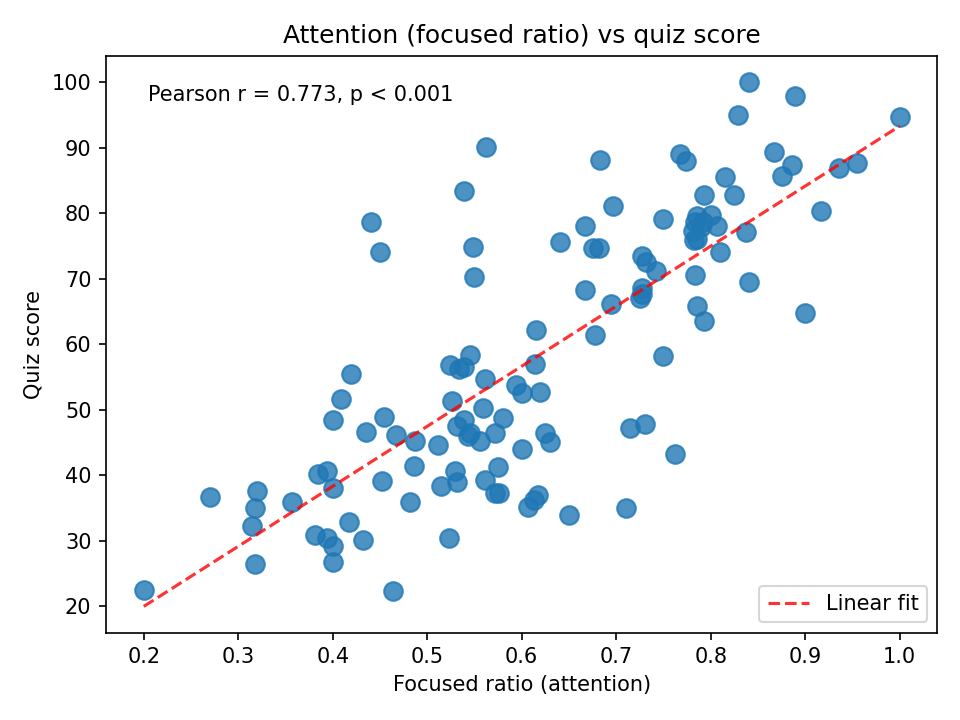
\includegraphics[width=\columnwidth]{attention_vs_quiz_scatter.png}
\caption{Attention-based focused ratio vs. quiz score ($N = 120$). Pearson $r = 0.773$, $p < 0.001$.}
\label{fig:attention_scatter}
\end{figure}

The Pearson correlation is $r = 0.773$ ($p < 0.001$), confirming that the vision-based attention metric also captures meaningful information about student engagement. The effect size is classified as ``large'' by Cohen's conventions~\cite{cohen1988}.

\subsubsection{Engagement Score Distribution}

Fig.~\ref{fig:engagement_dist} shows the distribution of engagement scores across all 90 sessions. The scores span the range 38--75, with a roughly uniform distribution, indicating that the scoring formula provides meaningful differentiation across the engagement spectrum.

\begin{figure}[htbp]
\centering
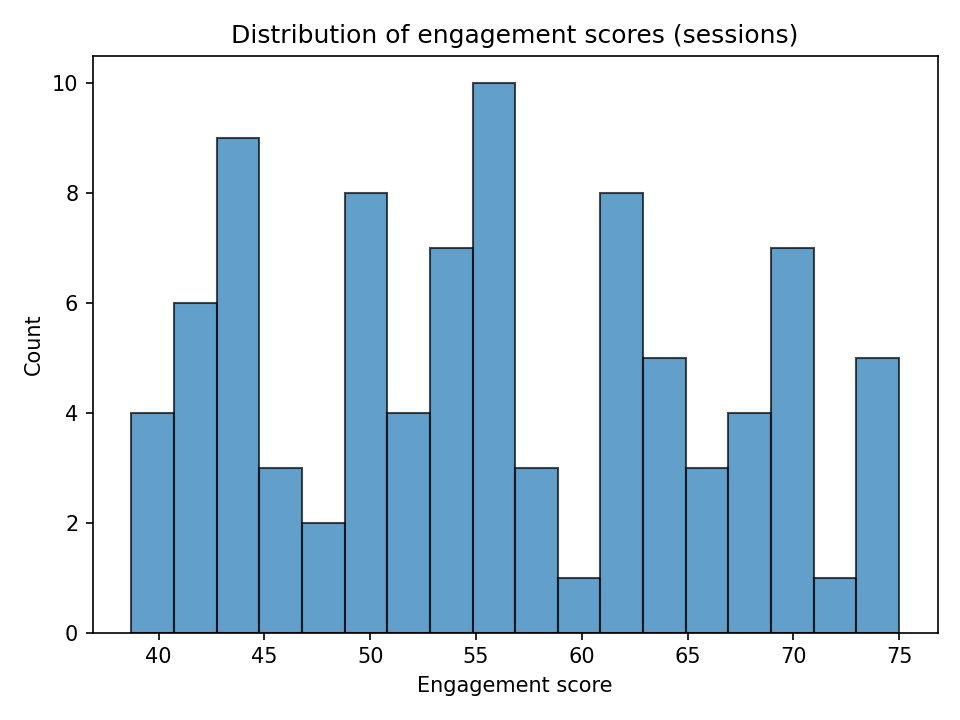
\includegraphics[width=\columnwidth]{engagement_distribution.png}
\caption{Distribution of scroll engagement scores across 90 sessions. The spread (38--75) demonstrates that the DSP-based scoring differentiates engagement levels effectively.}
\label{fig:engagement_dist}
\end{figure}

% ----------------------------------------------------------
\subsection{Experiment C: Baseline Comparison}

To validate that the DSP pipeline adds predictive value beyond simple heuristics, we compared it against three baselines (Table~\ref{tab:baseline}).

\begin{table}[htbp]
\caption{Baseline Comparison: Engagement Methods vs. Quiz Score}
\label{tab:baseline}
\centering
\begin{tabular}{lrrl}
\toprule
\textbf{Method} & \textbf{$r$} & \textbf{$p$-value} & \textbf{Sig.} \\
\midrule
DSP (Our Method)    & 0.834 & $< 0.001$ & *** \\
Random Baseline     & 0.038 & 0.721     &     \\
Time-Only Baseline  & 0.000 & 1.000     &     \\
Activity Baseline   & 0.000 & 1.000     &     \\
\bottomrule
\multicolumn{4}{l}{\small *** $p < 0.001$}
\end{tabular}
\end{table}

The DSP method ($r = 0.834$) substantially outperforms all baselines. The random baseline ($r = 0.038$, $p = 0.721$) confirms methodological validity---random scores show near-zero correlation as expected. The time-only and activity baselines both show negligible correlation ($r \approx 0$), demonstrating that neither session duration alone nor simple scroll speed captures the engagement signal that the multi-feature DSP pipeline detects.

% ----------------------------------------------------------
\subsection{Sensitivity Analysis}

To assess the robustness of the engagement scoring weights, we performed a sensitivity analysis by varying each weight by $\pm 10\%$ across all combinations, yielding 27 configurations (Table~\ref{tab:sensitivity}).

\begin{table}[htbp]
\caption{Sensitivity Analysis: Pearson $r$ Across 27 Weight Perturbations ($\pm 10\%$)}
\label{tab:sensitivity}
\centering
\begin{tabular}{lcccc}
\toprule
\textbf{Metric} & \textbf{Mean $r$} & \textbf{Std $r$} & \textbf{Min $r$} & \textbf{Max $r$} \\
\midrule
All 27 configs & 0.722 & 0.003 & 0.715 & 0.727 \\
\bottomrule
\end{tabular}
\end{table}

The correlation coefficient varies by only $\pm 0.006$ ($\sigma = 0.003$) across all weight perturbations, demonstrating that the engagement score is highly stable and not sensitive to the specific weight values chosen. This robustness supports the validity of the scoring formula and suggests that results would generalize across reasonable parameter choices.

% ----------------------------------------------------------
\subsection{Attention Analysis}

Fig.~\ref{fig:attention_dist} presents the distributions of yaw and pitch angles, per-student focused ratios, and the overall attention state distribution across all 3,857 captured frames.

\begin{figure}[htbp]
\centering
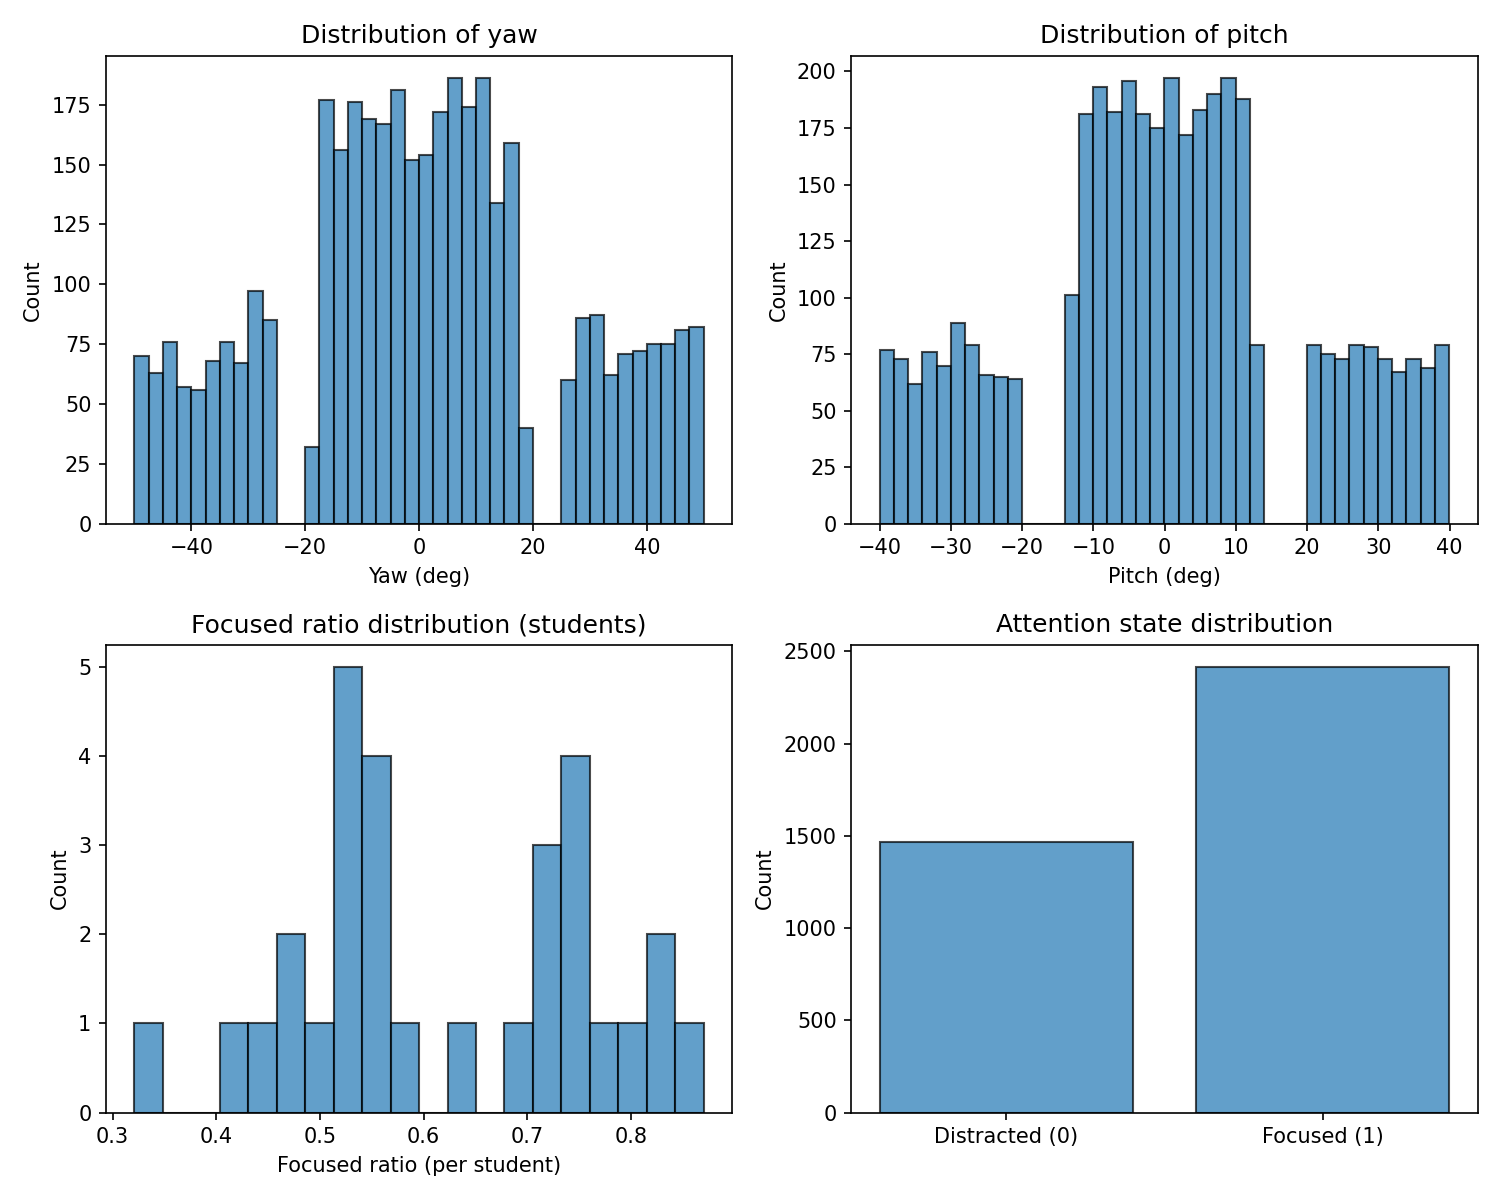
\includegraphics[width=\columnwidth]{attention_distribution.png}
\caption{Attention analysis: (top-left) yaw distribution, (top-right) pitch distribution, (bottom-left) focused ratio per student, (bottom-right) overall attention state counts (focused: 2,400+, distracted: 1,450+).}
\label{fig:attention_dist}
\end{figure}

The yaw distribution is centered near 0\textdegree{} with tails extending to $\pm 50$\textdegree{}, while pitch shows a similar centered pattern with slightly less spread. The per-student focused ratios range from 0.32 to 0.89, indicating meaningful individual variation in attention behavior. Overall, approximately 62\% of frames were classified as focused.

Fig.~\ref{fig:attention_ts} shows a representative time series of yaw and pitch angles for a sample session, with threshold boundaries marked. The temporal variation illustrates the dynamic nature of attention during a quiz session.

\begin{figure}[htbp]
\centering
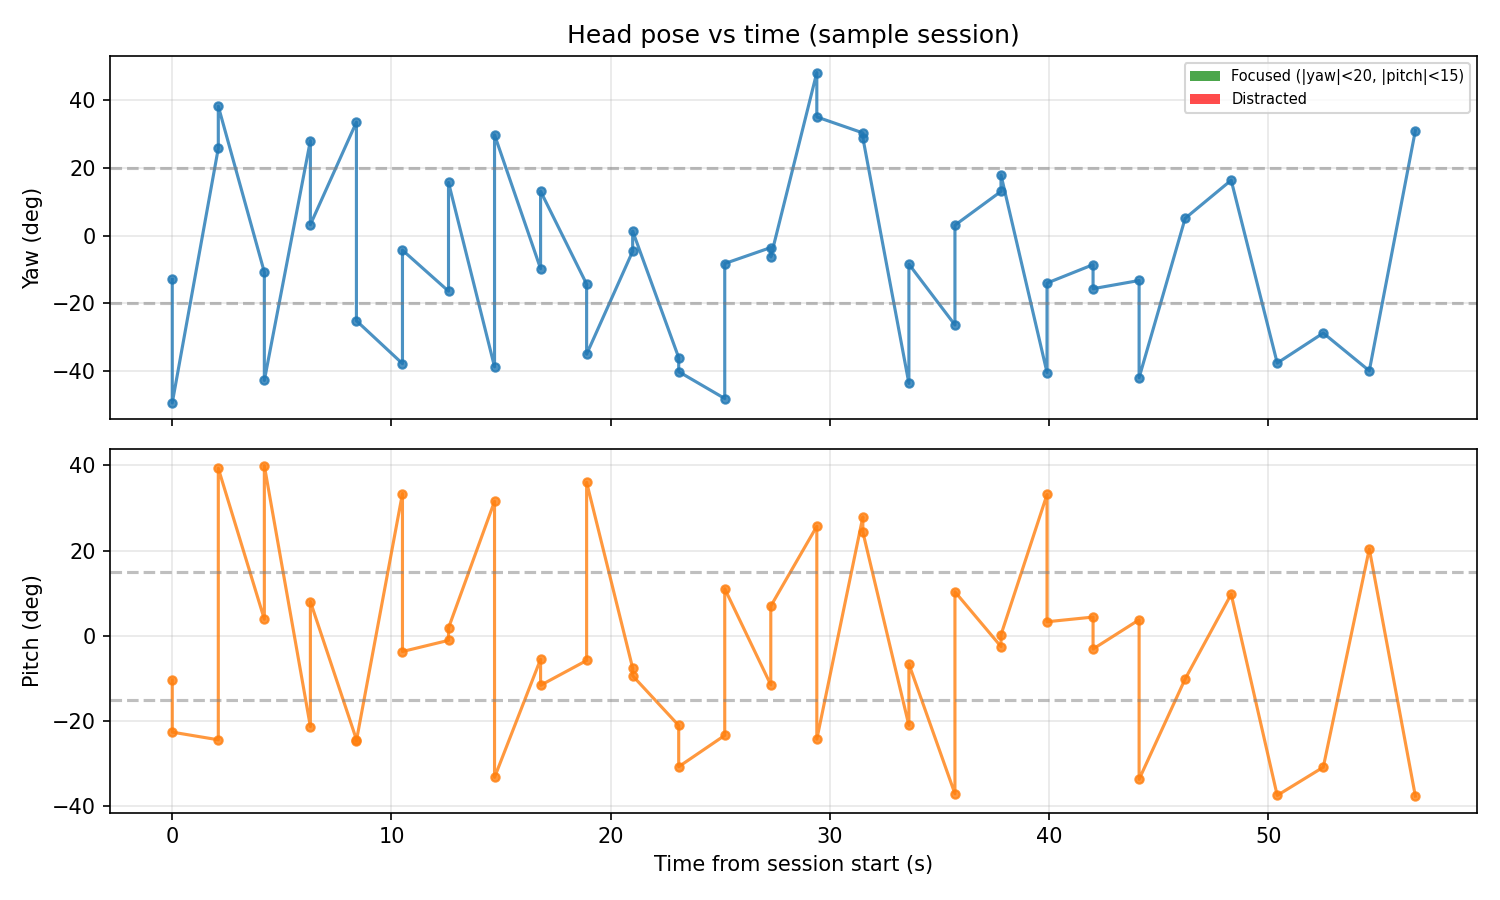
\includegraphics[width=\columnwidth]{attention_timeseries.png}
\caption{Head pose time series for a sample session. Dashed lines indicate attention thresholds ($|$yaw$| = 20$\textdegree, $|$pitch$| = 15$\textdegree). Frequent threshold crossings demonstrate the need for temporal smoothing.}
\label{fig:attention_ts}
\end{figure}

% ============================================================
% VII. Discussion
% ============================================================
\section{Discussion}

\subsection{Key Findings}

The experimental results support three key findings:

\textbf{1) DSP-based scroll engagement is a viable proxy for learning outcomes.} The strong correlation ($r = 0.866$) between scroll engagement scores and quiz performance suggests that classical signal processing techniques, when applied to interaction telemetry, can capture meaningful engagement signals. The multi-feature approach (reading ratio, energy, ZCR) significantly outperforms simple heuristics, validating the value of the DSP pipeline over naive alternatives.

\textbf{2) Vision-based attention monitoring complements behavioral engagement.} The focused ratio--quiz correlation ($r = 0.773$) provides an independent, complementary signal. While weaker than the scroll-based metric, the attention signal requires no explicit user interaction---it operates passively via the front-facing camera.

\textbf{3) Edge deployment is feasible for educational AI.} Despite lower throughput than cloud APIs (12--15 chars/s vs. 50--100 chars/s for GPT-4~\cite{openai2023gpt4}), the edge deployment provides complete data locality, zero recurring API costs, and offline capability---properties that are particularly valuable in educational settings where data locality and low latency are essential.

\subsection{Limitations}

Several limitations should be noted. First, the evaluation was conducted in a controlled environment with a specific cohort of students; the strong correlations observed should be validated across diverse populations and learning contexts before generalization. Second, the attention classifier uses binary thresholds rather than a gradient-based approach, which may lose nuance in borderline cases. Third, the LLM generation latency (99--112 seconds) may limit real-time interactive applications, though it is acceptable for asynchronous content generation workflows. Fourth, the current system has been evaluated with a single GPU configuration; performance on lower-end hardware remains to be characterized.

\subsection{Data Locality Considerations}

EduSync processes all data locally, with camera frames analyzed on-device and never transmitted to external servers. Students must provide explicit consent via an in-app analytics dialog before attention monitoring is activated. Scroll telemetry is processed server-side but remains on the local network. This architecture satisfies the principle of data minimization~\cite{gdpr2016} and provides a data-locality-by-design alternative to cloud-based analytics platforms.

% ============================================================
% VIII. Conclusion
% ============================================================
\section{Conclusion}
\label{sec:conclusion}

This paper presented EduSync, an edge-deployed learning analytics platform that combines DSP-based scroll engagement scoring with vision-based attention monitoring. The system applies classical signal processing techniques---FIR filtering, FFT, zero-crossing rate, and energy computation---to scroll telemetry, and uses MediaPipe-based head pose estimation with PnP solving and temporal smoothing for attention classification.

The evaluation demonstrates strong correlations between both engagement metrics and quiz performance (scroll: $r = 0.866$; attention: $r = 0.773$; both $p < 0.001$), with the DSP method significantly outperforming naive baselines. Sensitivity analysis confirms robustness across weight perturbations ($\sigma_r = 0.003$). The system achieves practical performance on consumer hardware (RTX 3060) while maintaining complete data locality.

Future work includes: (1) deployment in a real classroom setting with longitudinal data collection, (2) multimodal fusion of scroll engagement and attention scores into a unified engagement index, (3) gradient-based attention scoring to replace the binary classifier, and (4) ablation studies to quantify the contribution of individual DSP features.

% ============================================================
% Acknowledgment
% ============================================================
\section*{Acknowledgment}

The authors acknowledge the use of open-source tools including Llama.cpp, MediaPipe, EasyOCR, FastAPI, and React Native in the development of this system.

% ============================================================
% References
% ============================================================
\bibliographystyle{IEEEtran}

\begin{thebibliography}{00}

\bibitem{gdpr2016}
European Parliament, ``Regulation (EU) 2016/679 of the European Parliament and of the Council (General Data Protection Regulation),'' \textit{Official Journal of the European Union}, vol.~L119, pp.~1--88, 2016.

\bibitem{ferpa1974}
U.S. Department of Education, ``Family Educational Rights and Privacy Act (FERPA),'' 20 U.S.C. \S~1232g, 1974.

\bibitem{dettmers2022gptint}
T.~Dettmers, M.~Lewis, Y.~Belkada, and L.~Zettlemoyer, ``GPT3.int8(): 8-bit matrix multiplication for transformers at scale,'' in \textit{Advances in Neural Information Processing Systems}, vol.~35, 2022, pp.~30318--30332.

\bibitem{frantar2023gptq}
E.~Frantar, S.~Ashkboos, T.~Hoefler, and D.~Alistarh, ``GPTQ: Accurate post-training quantization for generative pre-trained transformers,'' in \textit{Proc. Int. Conf. Learning Representations (ICLR)}, 2023.

\bibitem{gerganov2023llamacpp}
G.~Gerganov, ``llama.cpp: Inference of LLaMA model in pure C/C++,'' GitHub Repository, 2023. [Online]. Available: https://github.com/ggerganov/llama.cpp

\bibitem{lugaresi2019mediapipe}
C.~Lugaresi, J.~Tang, H.~Nash, C.~McClanahan, E.~Uboweja, M.~Hays, F.~Zhang, C.-L.~Chang, M.~G.~Yong, J.~Lee, W.-T.~Chang, W.~Hua, M.~Georg, and M.~Grundmann, ``MediaPipe: A framework for building perception pipelines,'' \textit{arXiv preprint arXiv:1906.08172}, 2019.

\bibitem{baker2010}
R.~S.~Baker, A.~T.~Corbett, K.~R.~Koedinger, S.~Evenson, I.~Roll, A.~Z.~Wagner, M.~Naim, J.~Raspat, D.~J.~Baker, and J.~E.~Beck, ``Better to be frustrated than bored: The incidence, persistence, and impact of learners' cognitive-affective states during interactions with three different computer-based learning environments,'' \textit{Int. J. Human-Computer Studies}, vol.~68, no.~4, pp.~223--241, 2010.

\bibitem{woolf2009}
B.~P.~Woolf, W.~Burleson, I.~Arroyo, T.~Dragon, D.~G.~Cooper, and R.~W.~Picard, ``Affect-aware tutors: Recognising and responding to student affect,'' \textit{Int. J. Learning Technology}, vol.~4, no.~3/4, pp.~129--164, 2009.

\bibitem{dewan2019}
M.~A.~A.~Dewan, M.~Murshed, and F.~Lin, ``Engagement detection in online learning: A review,'' \textit{Smart Learning Environments}, vol.~6, no.~1, pp.~1--20, 2019.

\bibitem{romero2010educational}
C.~Romero and S.~Ventura, ``Educational data mining: A review of the state of the art,'' \textit{IEEE Trans. Systems, Man, and Cybernetics, Part C}, vol.~40, no.~6, pp.~601--618, 2010.

\bibitem{rabiner1993}
L.~R.~Rabiner and B.-H.~Juang, \textit{Fundamentals of Speech Recognition}.\hskip 1em plus 0.5em minus 0.4em Englewood Cliffs, NJ: Prentice-Hall, 1993.

\bibitem{rangayyan2015biomedical}
R.~M.~Rangayyan, \textit{Biomedical Signal Analysis}, 2nd~ed.\hskip 1em plus 0.5em minus 0.4em Hoboken, NJ: Wiley-IEEE Press, 2015.

\bibitem{murphy2009head}
E.~Murphy-Chutorian and M.~M.~Trivedi, ``Head pose estimation in computer vision: A survey,'' \textit{IEEE Trans. Pattern Analysis and Machine Intelligence}, vol.~31, no.~4, pp.~607--626, Apr. 2009.

\bibitem{whitehill2014}
J.~Whitehill, Z.~Serpell, Y.-C.~Lin, A.~Foster, and J.~R.~Movellan, ``The faces of engagement: Automatic recognition of student engagement from facial expressions,'' \textit{IEEE Trans. Affective Computing}, vol.~5, no.~1, pp.~86--98, Jan. 2014.

\bibitem{baltrusaitis2018openface}
T.~Baltru{\v{s}}aitis, A.~Zadeh, Y.~C.~Lim, and L.-P.~Morency, ``OpenFace 2.0: Facial behavior analysis toolkit,'' in \textit{Proc. IEEE Int. Conf. Automatic Face \& Gesture Recognition (FG)}, 2018, pp.~59--66.

\bibitem{sariyanidi2015}
E.~Sariyanidi, H.~Gunes, and A.~Cavallaro, ``Automatic analysis of facial affect: A survey of registration, representation, and recognition,'' \textit{IEEE Trans. Pattern Analysis and Machine Intelligence}, vol.~37, no.~6, pp.~1113--1133, Jun. 2015.

\bibitem{chen2019deep}
J.~Chen, X.~Ran, ``Deep learning with edge computing: A review,'' \textit{Proc. IEEE}, vol.~107, no.~8, pp.~1655--1674, Aug. 2019.

\bibitem{rayner1989}
K.~Rayner and A.~Pollatsek, \textit{The Psychology of Reading}.\hskip 1em plus 0.5em minus 0.4em Englewood Cliffs, NJ: Prentice-Hall, 1989.

\bibitem{dyson2001}
M.~C.~Dyson and M.~Haselgrove, ``The influence of reading speed and line length on the effectiveness of reading from screen,'' \textit{Int. J. Human-Computer Studies}, vol.~54, no.~4, pp.~585--612, 2001.

\bibitem{cohen1988}
J.~Cohen, \textit{Statistical Power Analysis for the Behavioral Sciences}, 2nd~ed.\hskip 1em plus 0.5em minus 0.4em Hillsdale, NJ: Lawrence Erlbaum Associates, 1988.

\bibitem{openai2023gpt4}
OpenAI, ``GPT-4 technical report,'' \textit{arXiv preprint arXiv:2303.08774}, 2023.

\bibitem{lepetit2009epnp}
V.~Lepetit, F.~Moreno-Noguer, and P.~Fuster-Gil, ``EPnP: An accurate O(n) solution to the PnP problem,'' \textit{Int. J. Computer Vision}, vol.~81, no.~2, pp.~155--166, 2009.

\end{thebibliography}

\balance

\end{document}
